\section*{Algorithms}

The algorithm used is the penalty method. The outer constrained
problem is converted into a sequence of unconstrained problems with the objective
\[
    \phi(x) = f(x) + \rho_1 \sum_i \mathbf{1}\{c_i(x)>0\}
        + \rho_2 \sum_i \max(c_i(x),0)^2
\]
The inner unconstrained problem is solved with normalized gradient descent and
backtracking line search. The gradient used by the inner method is
\[
    \nabla \phi(x) \approx \nabla f(x)
        + 2\rho_2 J_c(x)^T \max(c(x),0)
\]
where the constraint Jacobian \(J_c(x)\) is estimated by forward finite differences.
The count penalty is included in the objective value, but not in the gradient because
it is piecewise constant and has zero gradient almost everywhere.

For all five problems I used the same method with \(\rho_1=1\), \(\rho_2=10\), and
\(\gamma=4\), where both penalty weights are multiplied by \(\gamma\) after each outer
penalty iteration.  The inner minimization is capped at five accepted descent steps.
This cap was chosen empirically: it gives the outer loop frequent chances to increase
the penalty weights instead of spending the whole evaluation budget optimizing a weak
early penalty objective.

\textbf{Why it works.}  Violated constraints add a positive penalty, so descent on
\(\phi\) pushes iterates toward feasibility.  Increasing \(\rho_1\) and \(\rho_2\)
makes feasibility more important over time.  The finite-difference Jacobian gives the
method a local direction for reducing constraint violation without hard-coding any
constraint gradients.

\textbf{Pros.}  The method is generic, uses only \(f\), \(g\), and \(c\), and works for
the simple problems as well as higher-dimensional secret problems because the
constraints are flattened before computing violations.

\textbf{Cons.}  The method spends extra evaluations estimating \(J_c(x)\).  It is also
sensitive to penalty scaling: if the penalty is too weak, feasibility improves slowly;
if it is too strong, the penalty term can dominate the original objective.

For comparison plots, I used a pure quadratic penalty
\[
    \phi_q(x) = f(x) + \rho_2 \sum_i \max(c_i(x),0)^2
\]

\section*{Feasible Regions and Paths}

For \texttt{simple1}, both methods move the iterates from initially infeasible or
weakly feasible points toward the green feasible set.  The mixed penalty tends to
push more directly toward feasibility because the count penalty changes the line
search objective whenever a constraint remains violated.

\begin{figure}[H]
    \centering
    \begin{subfigure}{0.48\linewidth}
        \centering
        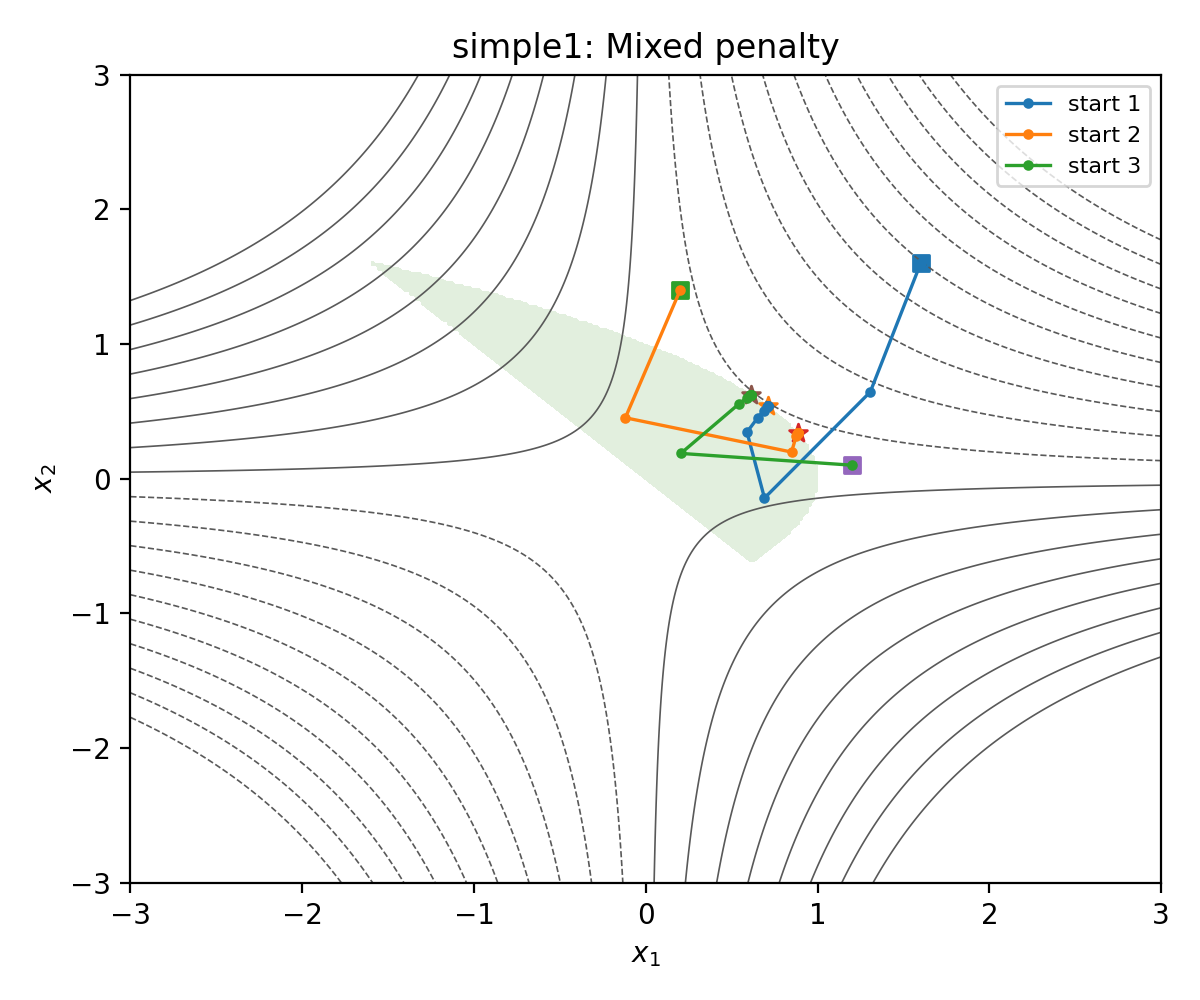
\includegraphics[width=\linewidth]{img/simple1_mixed_path.png}
        \caption{\texttt{simple1}, mixed penalty}
    \end{subfigure}
    \hfill
    \begin{subfigure}{0.48\linewidth}
        \centering
        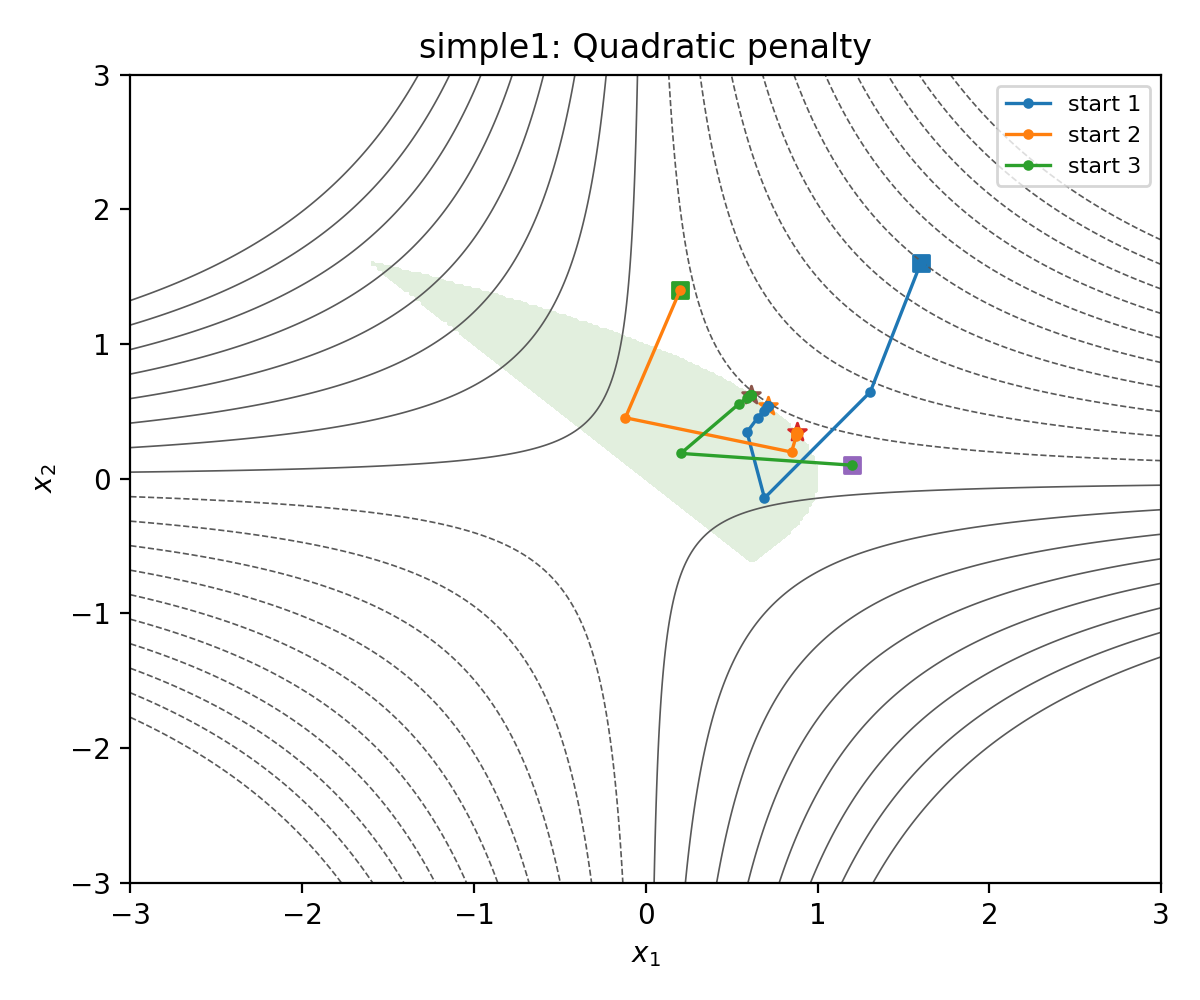
\includegraphics[width=\linewidth]{img/simple1_quadratic_path.png}
        \caption{\texttt{simple1}, quadratic penalty}
    \end{subfigure}
    \caption{Comparison of two penalty methods on \texttt{simple1}.}
\end{figure}

For \texttt{simple2}, the feasible region contains the constrained function
minimum near \((1,1)\).  The paths show the tradeoff between following the curved
function valley and reducing constraint violation; the penalty weights increasingly
favor feasibility as the outer iterations continue.
The paths are still visually similar because both methods use the same normalized
descent direction, and the count penalty does not contribute a useful smooth gradient.

\begin{figure}[H]
    \centering
    \begin{subfigure}{0.48\linewidth}
        \centering
        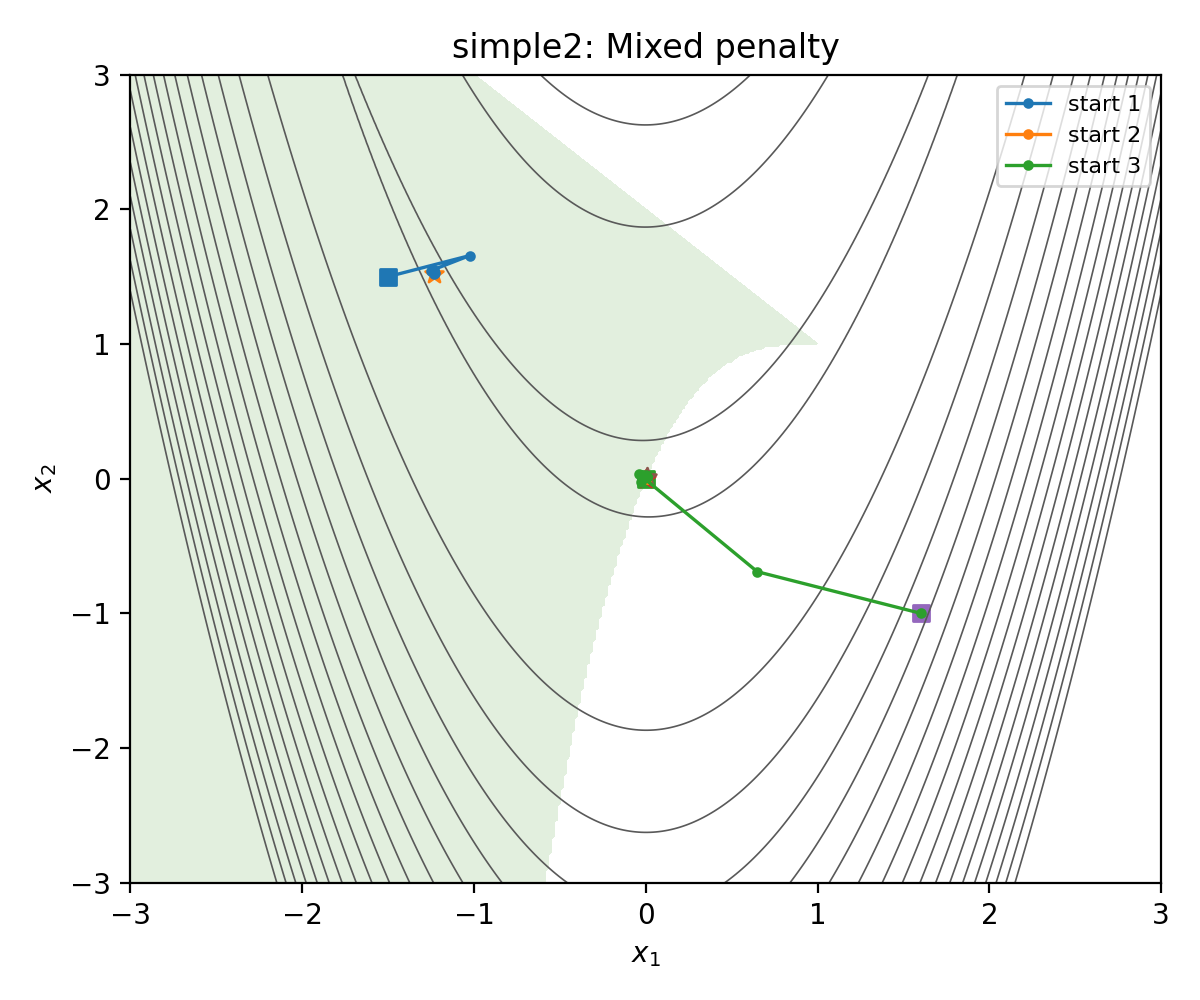
\includegraphics[width=\linewidth]{img/simple2_mixed_path.png}
        \caption{\texttt{simple2}, mixed penalty}
    \end{subfigure}
    \hfill
    \begin{subfigure}{0.48\linewidth}
        \centering
        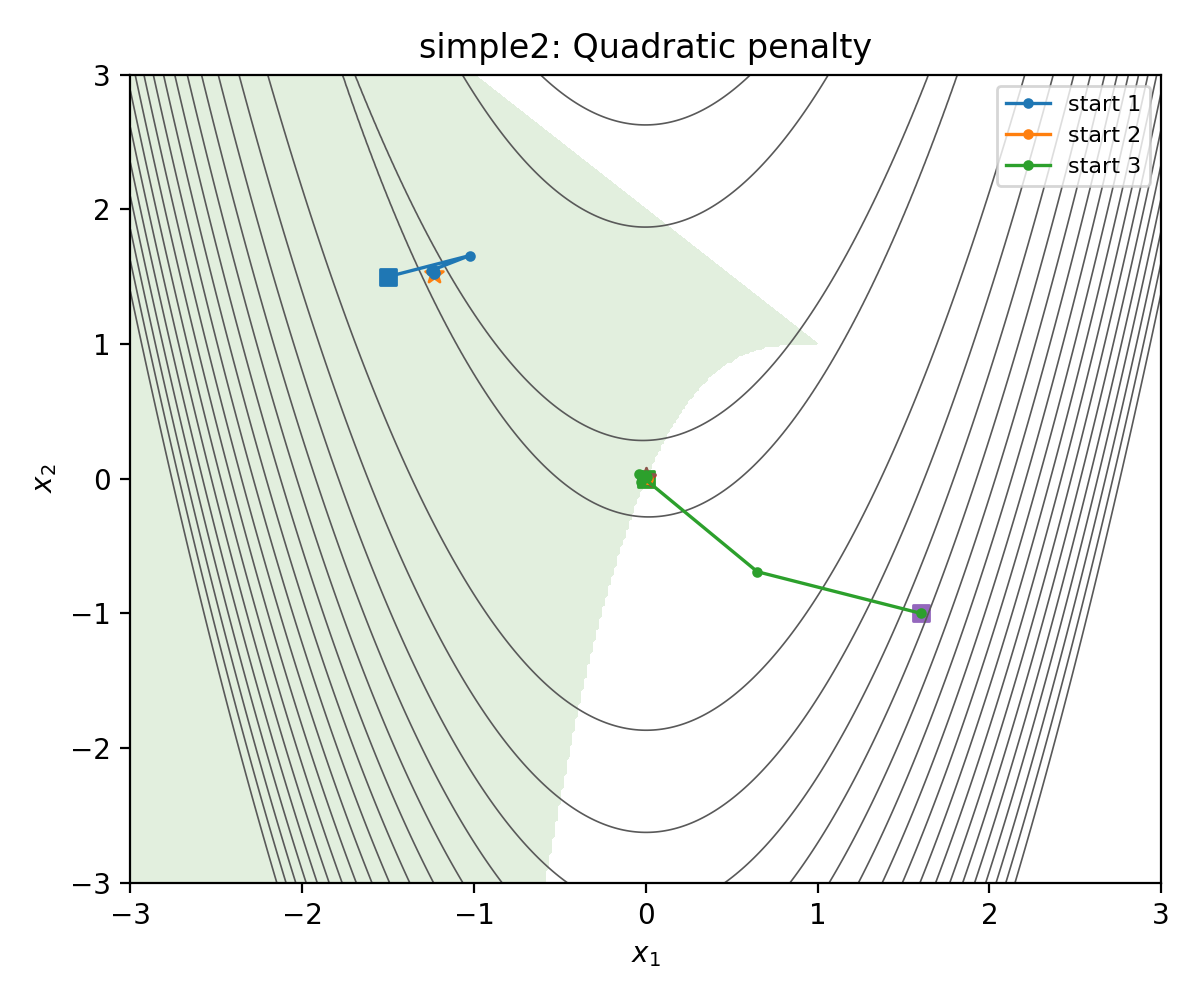
\includegraphics[width=\linewidth]{img/simple2_quadratic_path.png}
        \caption{\texttt{simple2}, quadratic penalty}
    \end{subfigure}
    \caption{Comparison of two penalty methods on \texttt{simple2}.}
\end{figure}

\section*{Convergence and Violation}

As plots indicate, the mixed penalty reduces the maximum violation more steadily.  The pure quadratic
penalty is more jagged on \texttt{simple2}, meaning some accepted steps move away
from feasibility before recovering.  For this problem, that makes the quadratic
penalty less reliable than the mixed penalty.

\begin{figure}[H]
    \centering
    \begin{subfigure}{0.48\linewidth}
        \centering
        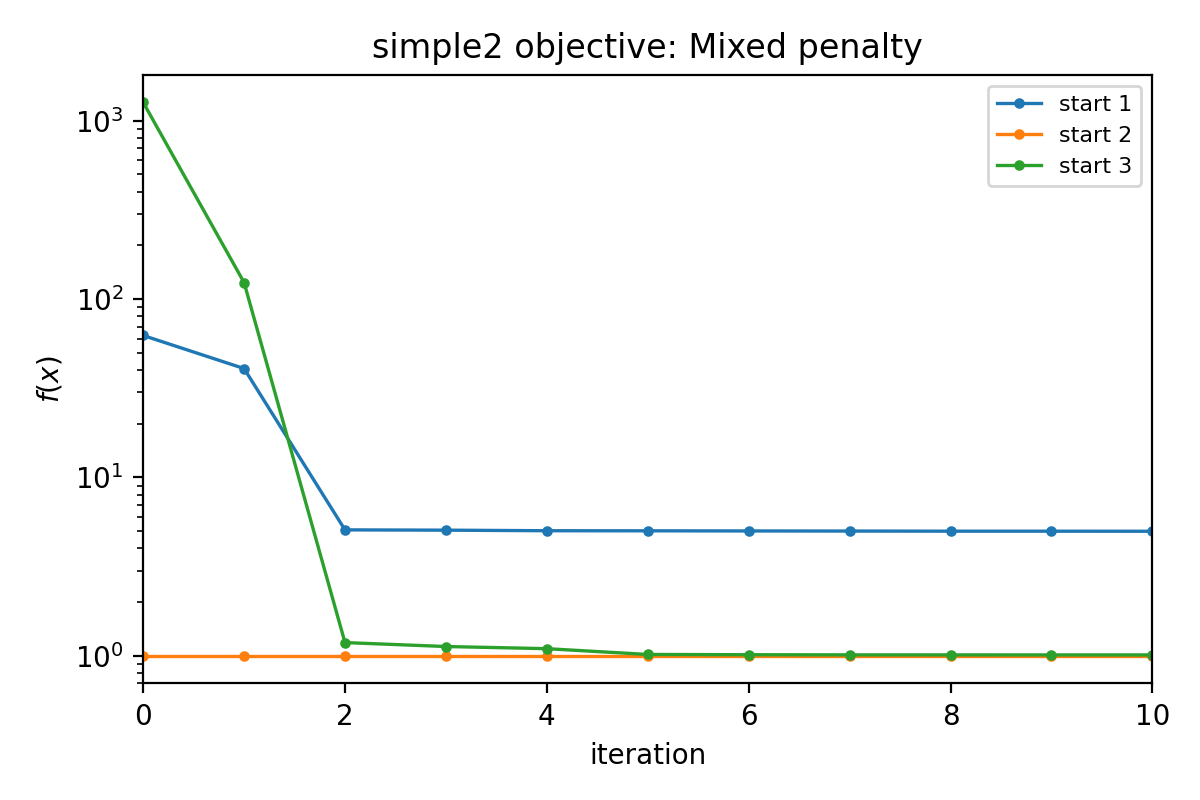
\includegraphics[width=\linewidth]{img/simple2_mixed_objective.png}
        \caption{Mixed penalty objective values}
    \end{subfigure}
    \hfill
    \begin{subfigure}{0.48\linewidth}
        \centering
        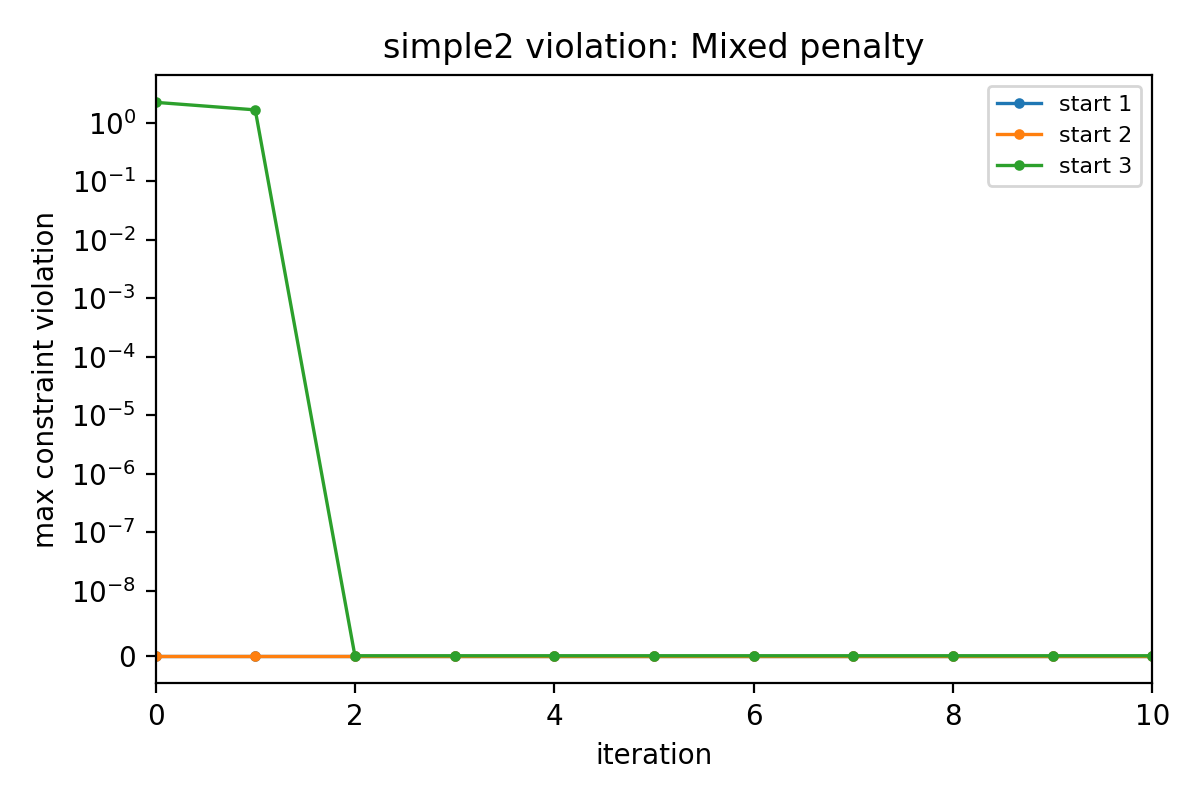
\includegraphics[width=\linewidth]{img/simple2_mixed_violation.png}
        \caption{Mixed penalty violation}
    \end{subfigure}
    \caption{\texttt{simple2} performance for the mixed penalty method.}
\end{figure}

\begin{figure}[H]
    \centering
    \begin{subfigure}{0.48\linewidth}
        \centering
        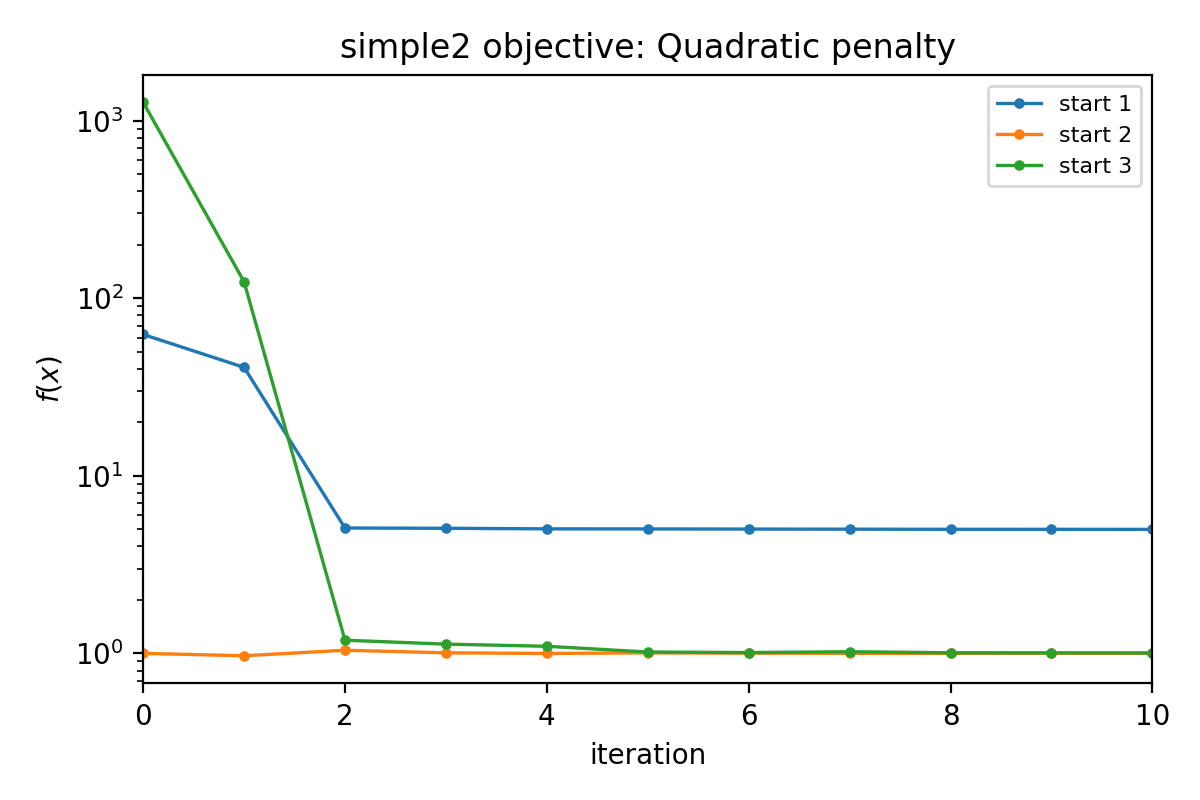
\includegraphics[width=\linewidth]{img/simple2_quadratic_objective.png}
        \caption{Quadratic penalty objective values}
    \end{subfigure}
    \hfill
    \begin{subfigure}{0.48\linewidth}
        \centering
        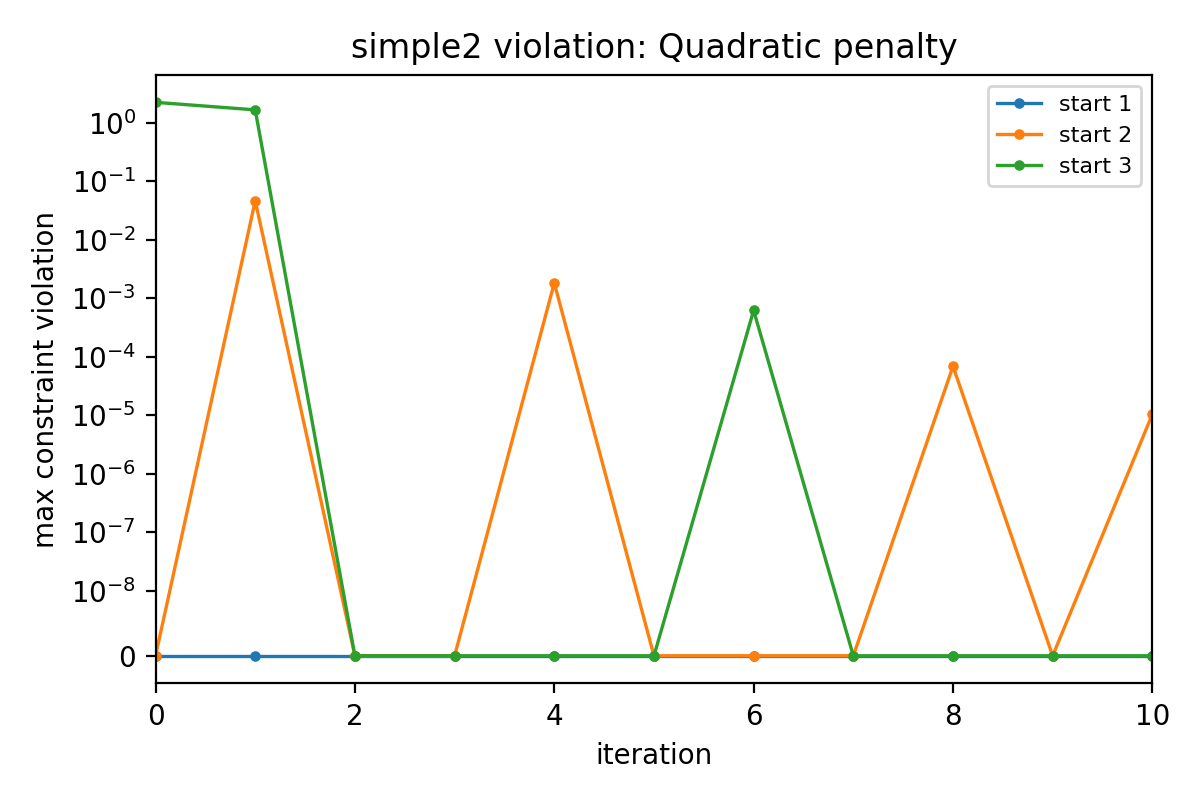
\includegraphics[width=\linewidth]{img/simple2_quadratic_violation.png}
        \caption{Quadratic penalty violation}
    \end{subfigure}
    \caption{\texttt{simple2} performance for the pure quadratic penalty method.}
\end{figure}

\section*{Code}

\begin{lstlisting}
def c_flat(c, x):
    return np.asarray(c(x), dtype=float).reshape(-1)

def descent_step(f, g, x, n, count):
    f_x = f(x)
    g_x = g(x)
    g_norm = np.linalg.norm(g_x)
    d = -g_x / g_norm

    alpha = 1.0
    p = 0.5
    beta = 1e-4

    while count() < n:
        x_trial = x + alpha * d
        f_trial = f(x_trial)
        if f_trial <= f_x + beta * alpha * (g_x.T @ d):
            return x_trial, True
        alpha *= p
    return x, False

def objective(x, f, c, rho1, rho2, n, count):
    if count() + 2 > n:
        return np.inf
    c_x = c_flat(c, x)
    p_count = np.sum(c_x > 0.0)
    p_quad = np.sum(np.maximum(c_x, 0.0) ** 2)
    return f(x) + rho1 * p_count + rho2 * p_quad

def grad_objective(x, f, g, c, rho2, n, count):
    if count() + 3 + len(x) > n:
        return None

    g_x = g(x)
    c_x = c_flat(c, x)
    m = np.maximum(c_x, 0.0)

    eps = 1e-6
    grad_c = np.zeros((len(c_x), len(x)))
    for j in range(len(x)):
        x_eps = x.copy()
        x_eps[j] += eps
        grad_c[:, j] = (c_flat(c, x_eps) - c_x) / eps

    return g_x + 2.0 * rho2 * (grad_c.T @ m)

def penalty_method(x0, f, g, c, n, count, rho1=1.0, rho2=10.0, gamma=4.0):
    x = x0.copy()
    best_x = x.copy()
    best_violation = np.inf

    while count() + 8 + len(x) <= n:
        x, _, _, _ = minimize(
            x,
            lambda z: objective(z, f, c, rho1, rho2, n, count),
            lambda z: grad_objective(z, f, g, c, rho2, n, count),
            n,
            count,
            max_steps=5,
        )

        c_x = c_flat(c, x)
        max_violation = np.max(np.maximum(c_x, 0.0))
        if max_violation < best_violation:
            best_x = x.copy()
            best_violation = max_violation
        if max_violation <= 0.0:
            return x

        rho1 *= gamma
        rho2 *= gamma

    return best_x
\end{lstlisting}
